\StartPlate{V31}{Keep the two construction routes distinct}{A source-defined candidate and a type-defined candidate require an identification theorem.}
\begin{center}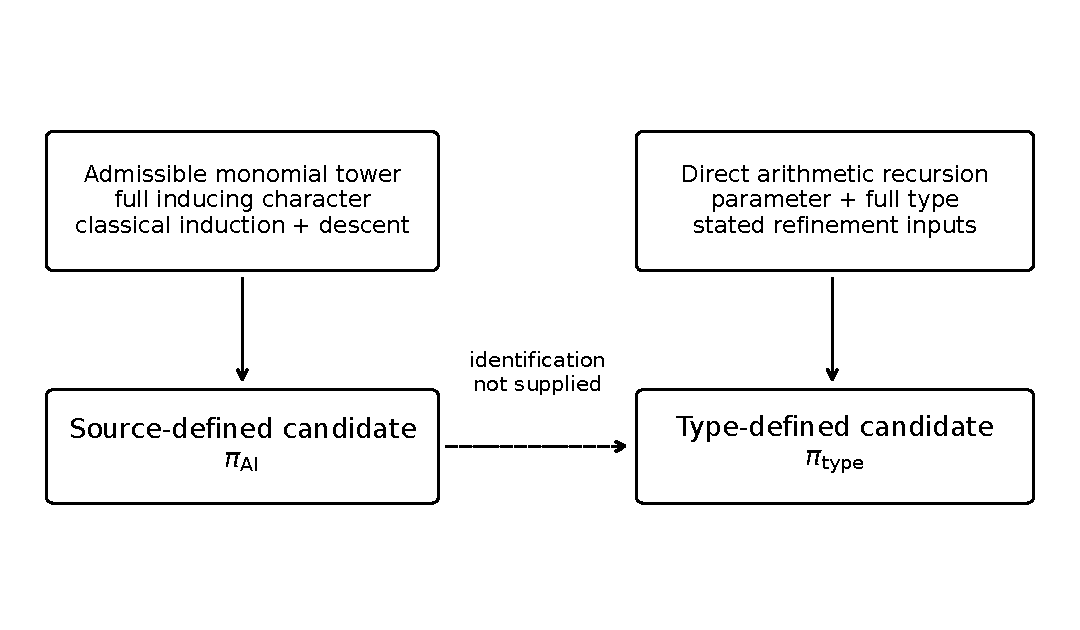
\includegraphics[width=\linewidth]{figures/V31.pdf}\end{center}
The monomial route begins with a full inducing character and an admissible tower. Under the stated classical induction and descent inputs it produces a source-defined candidate. Solvability of an ambient finite group does not make every proposed subgroup admissible for a prime-cyclic tower.

The direct route begins with an explicit parameter and type construction. Its refinement and full-character arguments produce an actual candidate under a restricted contract. Even when both routes match rank, standard conductor, torsion number, and self-pair conductor, those invariants do not identify their outputs.
\[
\pi_{\rm AI}\simeq\pi_{\rm type}
\quad\text{needs its own argument on the same source and field.}
\]
The positive-characteristic rank-nine source-defined route and the characteristic-zero continuation113 example remain separate cases. Neither is silently substituted for the other. The complete Henniart--Lemaire text was not freshly accessible in Block 4, so the detailed inherited theorem applications keep that audit boundary. This visual synthesis adds no new classical-source certification.
\vfill\PlateSource{Source-lineage diagram}{Part II, Sections 14 and 17; Part III, Section 25}{39}
